\section{The Setting} \label{sec:setting}

Modern data engineering and analysis techniques, spanning fields from classic statistics to medical research, rely heavily on predictive modeling. They revolve around examining observed datasets and building predictive models on outcomes of interest, based on a set of predictive features. A fundamental limitation of predictive models is their inability to capture the underlying generative mechanisms driving the relationships between the observed variables, relying purely on correlation statistics from observational data.

The well-known adage, \textit{Correlation does not imply causation}, exemplifies the fundamental challenge of causality, highlighting the need to move beyond predictive modeling and embrace causal reasoning. Importantly, the understanding of causal relationships is essential for answering “what-if” and “why” questions that go beyond mere prediction and association. In domains such as healthcare and climate change, one needs to know how an intervention (a change of the internal mechanisms of the examined system) will affect an outcome of interest, or even why a particular outcome occurred under certain observed conditions. In the end, for classical statistical and machine learning (ML) models, it all boils down to leveraging large portions of associational information and past experience from observational data, in order to construct, informally speaking, a pattern recognition system. 

Although so far in history predictive models have proven more than adequately robust for a wide range of applications, distributions of samples are assumed to be independent and identically distributed (i.i.d.), thus drawn from a single, unchanged distribution (samples are obtained under the same, unaltered experimental scenarios). What's more, understanding the underlying mechanism between cause and effect enables causal models to cover a wide range of distributions: By altering experimental conditions with interventions, one is able to uncover the true propagation of causation and perform reliable predictions under environmental changes. On the contrary, although statistical models have been proven robust for a variety of applications, they only account for modeling one general population distribution and are thus less interpretable. 

As an example, consider predicting ice cream sales based on the number of sunburn cases in a country. There clearly exists a correlation between these two observed quantities, so one may construct a model to predict ice cream sales based on its linear or non-linear relationship with sunburn cases. However, we generally know (taking it as expert knowledge) that the number of sunburn cases is not a cause of ice cream sales, but rather a result of the sun's radiation in the summer period. Allowing some gentle introduction to the appropriate terminology and notation, we qualitatively represent causal relationships of an underlying system using \textit{Directed Acyclic Graphs (DAGs)}\footnote{Other graphical structures exist, but are outside the scope of this work.}, where observed variables are depicted nodes and a directed edge \( X \rightarrow Y\) is interpreted as "\(X\) is a direct cause of \(Y\)" , while "\(Y\) a direct effect of \(X\)". With this in mind, the causal DAG described before is \(\text{Sun Radiation} \rightarrow Ice Cream Sales\) and \(\text{Sun Radiation} \rightarrow \text{Sunburn Cases}\).


Now imagine an alternate reality where the whole population is educated such that everyone applies adequate sunscreen before heading to the beach during summer. Using a model that performs its prediction trained on the false relationship discussed earlier in this modified population environment is guaranteed to produce highly inaccurate outcomes. This problematic case lies in the presence of the \textit{unobserved (latent) confounding variable} \( \text{Sun Radiation} \), which causally influences both \(\text{Sunburn Cases} \) and \( \text{Ice Cream Sales} \) (its direct children in the causal DAG). More often than not, creating a model that accounts for all possible eventualities is either impossible or intractable due to time or moral constraints. Of course, not all domains have been hindered by the observations we outlined, such as natural language processing (NLP), which has seen remarkable progress in recent years. Yet, our discussion so far further highlights the need for incorporating causality-based methods in machine learning algorithms to obtain a deeper understanding of examined systems. As \citet{scholkopf2021towards} point out: \\

\begin{chapquote}{\citet{scholkopf2021towards}}
``If we wish to incorporate learning algorithms into human decision making, we need to trust that the predictions of the algorithm will remain valid if the experimental conditions are changed.''
\end{chapquote}

As Reichenbach points out in the \textit{common cause principle} \citep{reichenbach1956direction}, if two variables \(X\) and \(Y\) are statistically dependent, then either (i) \(X\) causes \( Y\), (ii) \(Y\) causes \(X\) or importantly (iii) \textit{they share a common cause \(Z\) (a confounder \(X \leftarrow Z \rightarrow Y\)) that explains their association}. This principle lies at the heart of why observational data can be misleading: without accounting for all relevant variables, we risk attributing causal meaning to mere correlations. A classic illustration of this issue is \textit{Simpson's Paradox} \citep{simpson1951interpretation}, where trends apparent in aggregated data are reversed when disaggregated by a confounding variable. For instance, a treatment might appear beneficial in both men and women when analyzed separately, yet detrimental when the data is pooled together, due to the unequal distribution of underlying risk factors (e.g. a factor prominent in women).

Additionally, modern machine learning tools such as \textit{feature importance scores} and \textit{Shapley (SHAP) values} \citep{lundberg2017unified} often provide insights into which variables most strongly influence a prediction. Unfortunately, these measures are fundamentally \textit{associational} and non-causal: they capture how much a feature contributes to predictive accuracy within the model, but not whether the feature exerts a causal effect on the outcome. Consequently, they remain vulnerable to the same confounding phenomena highlighted previously: A variable may appear to have high importance or a strong SHAP attribution simply because it is correlated with an unobserved cause, rather than because it directly drives the outcome.

\begin{table}[ht!]
\centering
\caption{Comparison of different types of causal queries.}
\label{tab:causal-query-comparison}
\renewcommand{\arraystretch}{1.4}
\small
\begin{tabular}{|p{2.5cm}|p{2.5cm}|p{4cm}|p{2.5cm}|}
\hline
\textbf{Type} & \textbf{Notation} & \textbf{Interpretation} & \textbf{Data Source} \\
\hline
\textbf{Observational} & \( \mathbb{P}(Y \mid X=x) \) & How does \(Y\) vary when we observe \(X=x\)? & Observational \\
\hline
\textbf{Interventional} & \( \mathbb{P}(Y \mid \mathrm{do}(X=x)) \) & What happens to \(Y\) if we intervene and set \(X=x\)? & Interventional (RCTs, simulations) \\
\hline
\textbf{Counterfactual} & \( \mathbb{P}(Y_{X = x'} \mid X=x, Y=y, Z=z) \) & What would \(Y\) have been if \(X = x'\), given we saw \(X=x, Y=y, Z=z\)? & Model-based (SCMs + Abduction) \\
\hline
\end{tabular}
\end{table}

Given our discussion so far, how would one proceed to measure causal effects correctly? The gold standard since its introduction by Ronald Fisher \citep{fisher1935design}, has been with randomized experiments and more specifically with \textit{Randomized Control Trials (RCTs)}, where a subset of the examined population is randomly split into \textit{control} and \textit{treatment} groups, where one more more variables are deliberately manipulated (intervened) to isolate the causal effects being measured. As an illustrative example, consider a clinical trial where one needs to decide whether the newly introduced pill \(X\) prevents migraines. An RCT experiment would imply selecting a random patient sample, randomly splitting them into control (placebo pill) and treatment (pill \(X\)) groups and measure the causal effect of a quantity of interest (e.g. migraine pain level) on each group separately. The real magic of such controlled experiments lie in their ability to eliminate \textit{confounding bias} through randomization. By balancing both observed and unobserved covariates across groups, RCTs ensure that differences in outcomes are attributed solely to the intervention and not to systematic distortions caused by pre-existing conditions. In digital marketing and advertising campaigns, RCTs take the form of \textit{A/B tests}: users are randomly shown one of two versions of a webpage or a smartphone app (A or B) to determine which version has a greater causal effect on a desired outcome, such as \textit{click-through rate} or \textit{exposure rate} for a quantity of interest. Returning to our earlier ice cream and sunburn example, one would randomly assign a subset of the population to consume ice-cream (treatment group) and another to not (control group) and measure the causal effect of ice-cream consumption on sunburn cases. In formal terms, such a measurement can for example be the \textit{Average Treatment Effect (ATE)}, which is viewed as the expected difference in outcomes between treated and untreated populations: \(\text{ATE} = \mathbb{E}[Y_1 - Y_0]\) where \(Y_1\) and \(Y_0\) represent the potential outcomes under treatment and control, respectively. If this difference is statistically distinguishable from zero, one concludes that the treatment has a causal effect on the outcome.

However, controlled experiments like RCTs are often impractical due to cost, ethical constraints or logistical challenges, with many corporations running hundreds of them each day on their products. For instance, it would be prohibitive to force a population sample (including healthy individuals) to smoke for investigating whether smoking causes lung cancer. What is more, the space of possible A/B tests is combinatorial when one is considering combinations of several design choices or user behaviors, thus being unfeasible in practice. 

\begin{figure}[ht!]
\centering
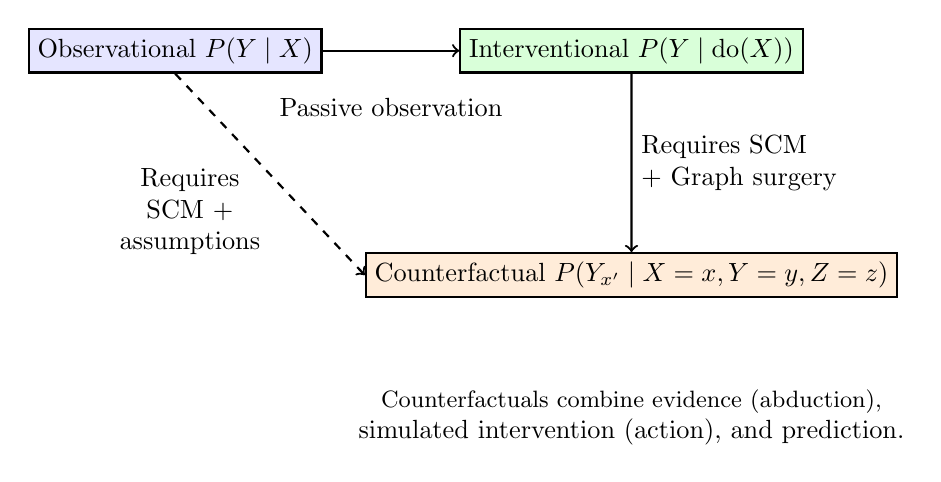
\begin{tikzpicture}[node distance=1.8cm, thick, every node/.style={scale=0.95}]
  % Nodes
  \node[draw, rectangle, fill=blue!10] (obs) {Observational \(\mathbb{P}(Y \mid X)\)};
  \node[draw, rectangle, fill=green!15, right of=obs, xshift=4.3cm] (intv) {Interventional \(\mathbb{P}(Y \mid \mathrm{do}(X))\)};
  \node[draw, rectangle, fill=orange!15, below of=intv, yshift=-1.2cm] (cf) {Counterfactual \(\mathbb{P}(Y_{x'} \mid X=x, Y=y, Z=z)\)};

  % Arrows
  \draw[->] (obs) -- node[below, yshift=-0.5cm] {Passive observation} (intv);
  \draw[->] (intv) -- node[right, align=left] {Requires SCM\\ + Graph surgery} (cf);
  \draw[->, dashed] (obs.south) -- node[left, align=center, yshift=-0.5cm] {Requires \\ SCM + \\ assumptions} (cf.west);

  % Labels
  \node[below of=cf, yshift=-0.1cm, align=center] (note) {\small Counterfactuals combine evidence (abduction),\\ simulated intervention (action), and prediction.};
\end{tikzpicture}
\caption{Illustration of the relationships and requirements between observational, interventional, and counterfactual causal queries.}
\label{fig:causal-query-flow}
\end{figure}

This is where the formal framework of \textit{Structural Causal Models (SCMs)} becomes essential. SCMs, introduced by Judea Pearl \citep{pearl2009causality} who pioneered the development of the theory of Causality (Turing Award 2011), offer a mathematical representation of the causal mechanisms that generate a dataset. In brief, an SCM consists of (i) a graph (in this text, a DAG) \(\mathcal{G}\) structure encoding the underlying causal relationships (ii) a set of structural equations (functional relationships) \( X_i := f_i (\text{Pa}_i, \epsilon_i)\) where \(\text{Pa}_i\) are the parents of \(X_i\) in the DAG and (iii) independent noise terms \(\epsilon_i\) representing unobserved randomness and possible confounders. In a nutshell, these structural equations \textit{encapsulate how each variable in a system is generated from its direct causes (parents in the DAG)}. The strength of such modeling lies in the ability to rigorously represent the causal mechanisms that generate a dataset, enabling the analysis of causal effects and interventions, and the estimation of causal quantities of interest, such as the ATE mentioned previously.

Furthermore, the concept of interventions is a fundamental operation in causal inference, formalized through \textit{do-calculus} by Pearl \citep{pearl1995causal}. The notation \(\mathbb{P}(Y|\text{do}(X=x))\) denotes the distribution of \(Y\) after an intervention on \(X\), directly setting its value to \(x\), irrespective of its natural causes. Such generated datasamples are called \textit{interventional data} in contrast to \textit{observational data} that are obtained from a purely observational perspective of the system. In terms of the SCM, this corresponds to \textit{graph surgery}: removing all incoming edges into \(X\) and replacing its value with a constant. This operation gives rise to a new graph, called the \textit{mutilated graph}, which simulates a world where we have forced \(X\) to be \(x\). This distinction is crucial because in observational data, one only has access to the conditional observational distribution \(\mathbb{P}(Y|X=x)\) which may be influenced by confounding or selection bias. On the other hand, the interventional distribution \(\mathbb{P}(Y|\text{do}(X=x))\) truly captures the causal effect of manipulating \(X\) on \(Y\). So generally, the interested reader may notice that \(\mathbb{P}(Y|X=x)\) (which may represent the outcome of a predictive model) is generally not equal to \( \mathbb{P}(Y|\text{do}(X=x))\)\footnote{They would be equal in the case of no backdoor-confounding path from \(X\) to \(Y\), but this is outside the scope of this thesis.}. Finally, a third important pillar in Causality is the concept of \textit{counterfactuals}, where one can quantify causal queries of the form \textit{"Given that I have observed \(X=0,Y=0\) and \(Z=1\), what would \(Y\) be if \(Z\) had been \(0\)?"}. That is, a counterfactual probability of the form \( \mathbb{P}(Y_{Z=0}=y|X=0, Y=0, Z=1)\). Computation of such queries is evaluated with a three-step procedure known as \textit{abduction}, \textit{action}, and \textit{prediction} using the known SCM \citep{pearl2009causality}. Here, \(Y_{Z=0}\) denotes the potential outcome representing the value that \(Y\) would have taken, in a reality where \(Z=1,X=0\) and \(Y=0\) have been observed. One concrete example of counterfactuals is: "Knowing that Hillary Clinton gave a speech in California and did not win the 2016 presidential election, would she had won had she not given that speech?". Unlike predictive explanations, which are conditional on inputs, counterfactuals model alternative realities rooted deeply in the structural model of the world, essential for decision-making under uncertainty and policy evaluation. Figure \ref{fig:causal-query-flow} and Table \ref{tab:causal-query-comparison} provides an overview of the causal queries discussed so far. 

In ML literature, one also encounters \textit{counterfactual explanations (CFEs)} \citep{guidotti2024counterfactual} which are commonly used as interpretability tools. These CFEs typically answer queries of the form "What minimal change in the input features would have altered the model's prediction?". One must note that they are not counterfactuals in the causal sense: they operate within the predictive model's input-output mapping, without assuming any underlying structural causal model. As a result, suggested changes may be infeasible, non-actionable, or causally meaningless. Table \ref{tab:causal-vs-predictive} provides an overview of the differences discussed between causal and predictive modeling.

\begin{table}[h!]
\centering
\renewcommand{\arraystretch}{1.2}
\begin{tabular}{|p{2.5cm}|p{5cm}|p{3cm}|p{3cm}|}
\hline
\textbf{Query} & \textbf{Description} & \textbf{Causal} & \textbf{Predictive} \\
\hline
Prediction & Predict/Diagnose $Y$ given $X$ & Correct predictions & Correct predictions \\
\hline
What-if & What if I set \(X_1=5\) ? & Correct prediction on $Y$ & Possibly wrong prediction on $Y$ \\
\hline
Decision Making & Optimal \(X_1\) to increase \(Y\) given \(X_2=6\) & Correct decisions & Possibly wrong decisions \\
\hline
Interpretation & Importance of \(X_1\) in affecting \(Y\); features influencing \(Y\) & Correct estimate & SHAP/feature importance may fail \\
\hline
Counterfactual & Example: \(Y=3\) when \(X_3=\) ``yellow''. What if \(X_3=\) ``green''? & Correct estimate & Not possible \\
\hline
Root Cause & What was the initial root cause of a failure? & Correct estimate & Possibly wrong estimates \\
\hline
\end{tabular}
\caption{Comparison of causal vs. predictive modeling across different types of queries.}
\label{tab:causal-vs-predictive}
\end{table}

All the above positive baggage of the theory of Causality is described by Judea Pearl in the \textit{3-step ladder of Causation} \citep{pearl2018book}. Any inference merely by observing associations lies in \textit{level 0} (as in statistical predictive models). The true power of causality belongs to interventions (\textit{level 1}) and counterfactuals (\textit{level 2}). From everyday choices to scientific inquiry, our actions are guided by the belief that certain causes will lead to specific effects. However, causality in real-world scenarios is often probabilistic rather than deterministic. As we have mentioned before, while smoking is a known cause of lung cancer, not all smokers develop the disease. This uncertainty is also where probability theory intersects with causal modeling, allowing us to quantify the likelihood of outcomes given specific causes.

%\begin{figure}[t!]
%\centering
%\begin{tikzpicture}[node distance=1.9cm]
%
%% Levels
%\node (seeing) [level] {Association (Seeing, Observing) \\ \(\mathbb{P}(Y \mid X)\)};
%\node (doing) [level, above=of seeing] {Interventions (Doing) \\ \(\mathbb{P}(Y \mid \mathrm{do}(X))\)};
%\node (imagining) [level, above=of doing] {Counterfactuals (Imagining, \textit{What if...}) \\ \( \mathbb{P}(Y_{x'} \mid X = x, Y = y, Z = z)\)};
%
%% Arrows
%\draw [arrow] (seeing) -- (doing);
%\draw [arrow] (doing) -- (imagining);
%
%% Labels
%\node [labelbox, right=0.6cm of seeing] {Observational ~Data};
%\node [labelbox, right=0.6cm of doing] {Interventional ~Data};
%\node [labelbox, right=0.6cm of imagining] {Abduction + SCM};
%
%\end{tikzpicture}
%\caption{Depiction of Pearl's Ladder of Causation, progressing from association (level 0) to intervention (level 1) and finally to counterfactual reasoning (level 2).}
%\label{fig:ladder-of-causation}
%\end{figure}

Overall, Causality can be split into two main research areas: \textit{causal discovery (CD)}, which aims to identify the true underlying causal relationships from data under certain assumptions and \textit{causal inference (CI)}, which concerns estimation and quantification of treatment effects without exhaustive experimentation. Formally, given a dataset \( \mathcal{D} \sim \mathcal{P}_{\mathcal{D}} \), the goal of causal discovery is to infer the underlying causal model \( \mathcal{G} \sim \mathcal{D} \). Methods developed for causal inference assume the ground truth causal structure as known. In practice, one starts by estimating the ground truth causal model using a causal discovery algorithm. Depending on the method, the discovered causal model may be paired with the estimated functional dependencies of the underlying SCM (e.g. some algorithms assume that data follow a linear generative process, so causal discovery is reduced to estimating the coefficients of the assumed linear model) or simply output the estimated DAG. In either case, one can use standard predictive models to estimate the functional relationships alongside valid adjustment sets to perform causal inference. This bridges causal discovery with interventional effect estimation: identifying optimal intervention strategies, computing ATEs, or performing counterfactual reasoning on outcomes of interest, as described previously. 

In recent years, significant attention has shifted on \textit{causal discovery for time-series (temporal) data} \citep{runge2018causal, runge2019inferring, runge2023causal}. For the unfamiliar reader, such samples are no longer considered i.i.d. as the time dimension is also present. Time-series are widely observed across a domain of environments, as long as data is collected across time intervals and exhibit a temporal order. For example, consider a time series of climate measurements (temperature, humidity, atmospheric pressure) over a day in a city, sampled every fifteen minutes. The resulting data is a sequence of three-dimensional 96 observations, and the corresponding (multivariate) time series is a time-series of length 96. Another concrete example would be a time series of stock prices, where data is collected every day for a year, resulting in a time series of length 365. For the most part, investigating causality for time-series consists as an extension of the theory developed for the static, i.i.d. counterparts, with some additional assumptions and complexities that arise from temporal dependencies, possible feedback loops, non-stationarity of the observed time-series, and unobserved confounding variables. Variables evolve over time, and causal influences can occur both contemporaneously (within the same time-index) and with various time lags (e.g. one day before). Without elaborating extensively in this part of the text, a \textit{contemporaneous} (or \textit{instantaneous}) relationship may occur if causal effects exist within an hourly period in an observed daily time-series. 

Concurrently and much to our benefit, there has been no previous period for ML and artificial intelligence (AI) with as much bloom and research opportunities. The current wave of interest, initiated with ML more than two decades ago and continued with \textit{deep learning (DL)} (the use of large neural network architectures for solving highly-complex, intractable tasks) has provided several radical solutions to numerous research questions, such as image recognition, that no previous AI period ever did. The witnessing of problems that have puzzled the scientific community for decades being deemed solved, like text-to-image generation, is an ongoing process. It is possible that since this ongoing take-off, the AI winter may not be coming anytime soon. 

Even more remarkably, causality for time-series data has only recently found large-scale applications in industrial domains, many years after Pearl's seminal contributions. Terms such as \textit{Causal AIOps} and \textit{Causal AI} correspond to complementing traditional machine learning with causal discovery \& causal inference methods, often based around modern neural architectures for industrial applications. Much to our excitement, \textit{Causal Digital Twins} \citep{jakovljevic2021towards} are also a promising direction, where a causal model is constructed from data to model a real-world system, to perform real-time causal inference and decision making. This enables tasks such as the identification of optimal interventional policies, which are crucial for understanding and correctly interpreting data-driven decisions. This paves exciting research paths for developing new state-of-the-art (SOTA) methods for causality on time-series for solving real-world problems.